\begin{figure}[!tbp]
    \centering
    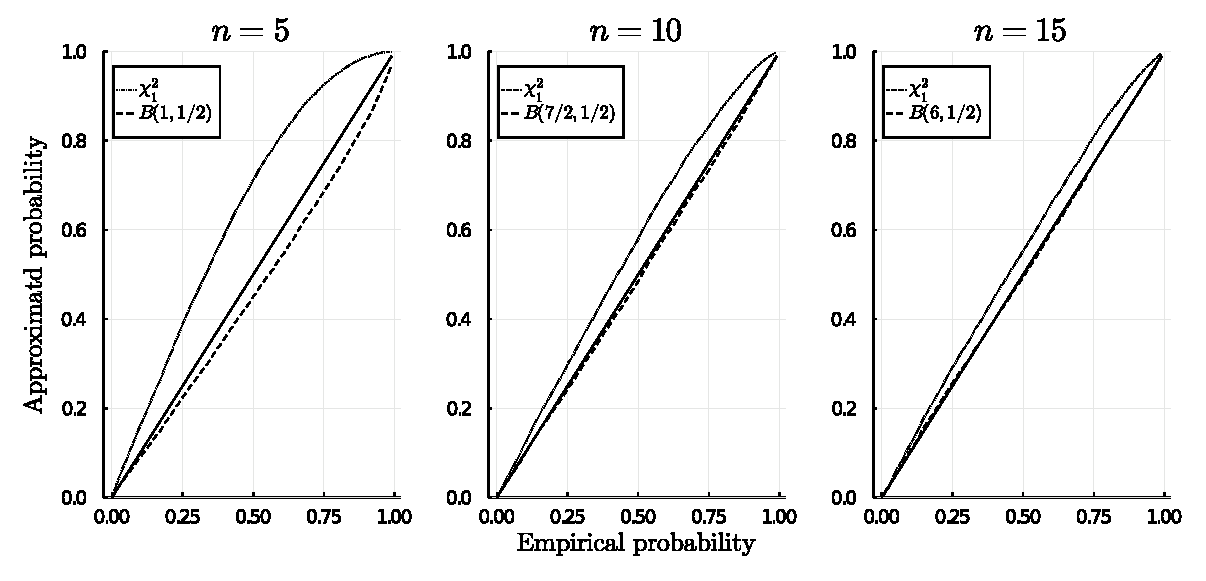
\includegraphics[width=16cm]{diamond_vs_square_0_1}
    \newline
    \newline
    \newline
    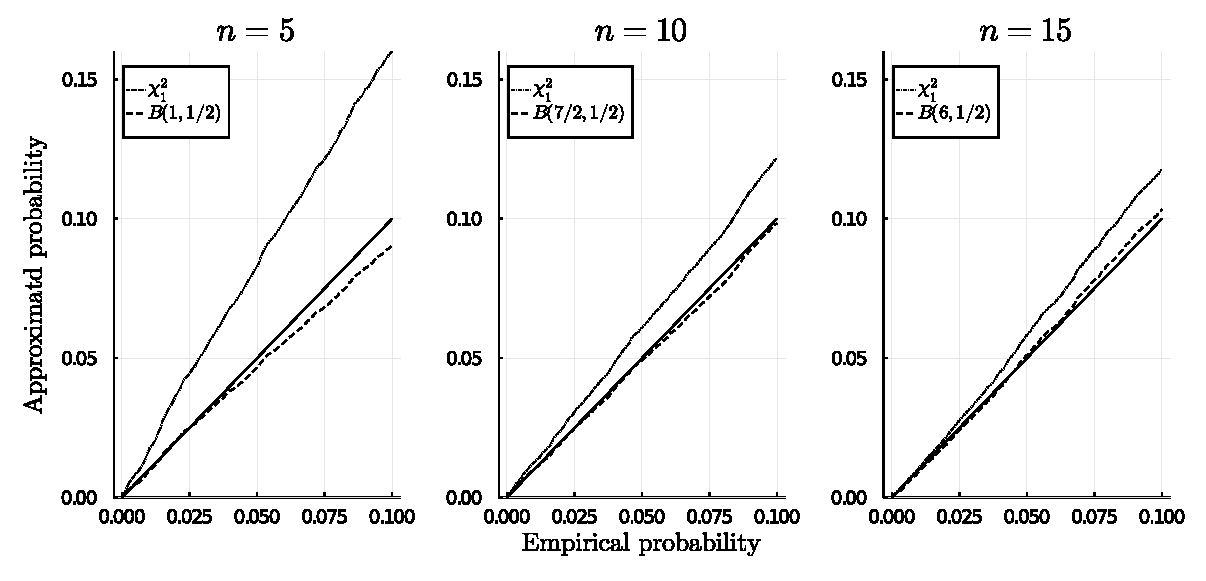
\includegraphics[width=16cm]{diamond_vs_square_0_01}
    \caption{Comparison of the $\chi^2_1$ approximation of the $\Lambda(S_n)$ statistic and Beta approximation of the $Q(S_n)$ statitistic from Eriksen \cite{eriksen1996tests} for testing the null hypothesis of a chordless cycle given a sample of $n = 5, 10, 15$ observations. As seen in the upper pane, the $\chi^2_1$ approximation poorly estimates the distribution of the $\Lambda(S_n)$ statistic for small and moderate sample sizes, while the $B((n - 3)/2, 1/2)$ approximation to the distribution of $Q(S_n)$ is accurate even for small sample sizes. This is particularly strong when focusing on small probability regions as we show in the lower pane where the difference of probability can be of approximately 50\%.}
    \label{fig-diamond-vs-square-small}
\end{figure}
